\documentclass[a4paper,10pt]{article}

\usepackage[ansinew]{inputenc}
\usepackage[spanish]{babel}
\usepackage{graphicx}
\usepackage{listings}
\usepackage{appendix}
\usepackage{pdfpages}
\usepackage{fancyhdr}
\pagestyle{fancy}

\begin{document}

\lhead{\fancyplain{}{Organizaci\'on de computadoras 66.20 - Turno Martes}}
\rhead{\fancyplain{}{Trabajo Pr\'actico 1}}

\setcounter{page}{2}

\newpage
\thispagestyle{empty}
\tableofcontents

\newpage
\section{Introducci\'on}
  TODO

\section{Resoluci\'on del problema}

  \subsection{Main unix2dos}
    \subsubsection{Stack frame}
      \begin{center}
	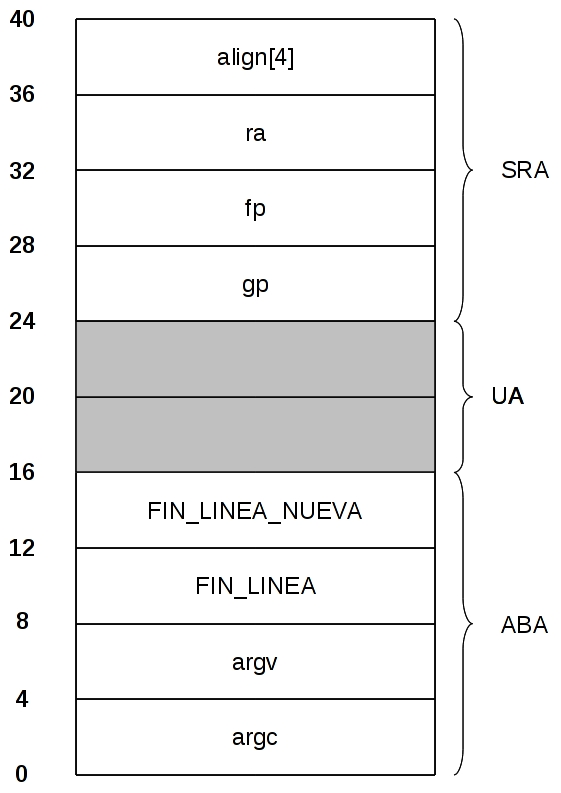
\includegraphics[width=10cm, height=15cm]{DibujosStackFrame/stack-unix2dos(main).jpg}
      \end{center}

  \subsection{Funci\'on parser}
    \subsubsection{Stack frame}
      \begin{center}
	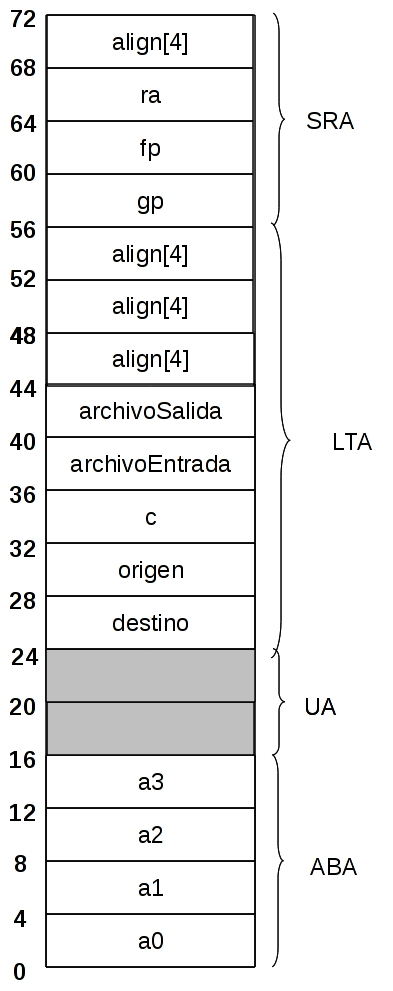
\includegraphics[width=11cm, height=16cm]{DibujosStackFrame/stack-parser.jpg}
      \end{center}

  \subsection{Funci\'on traducirFormato}
    \subsubsection{Stack frame}
      \begin{center}
	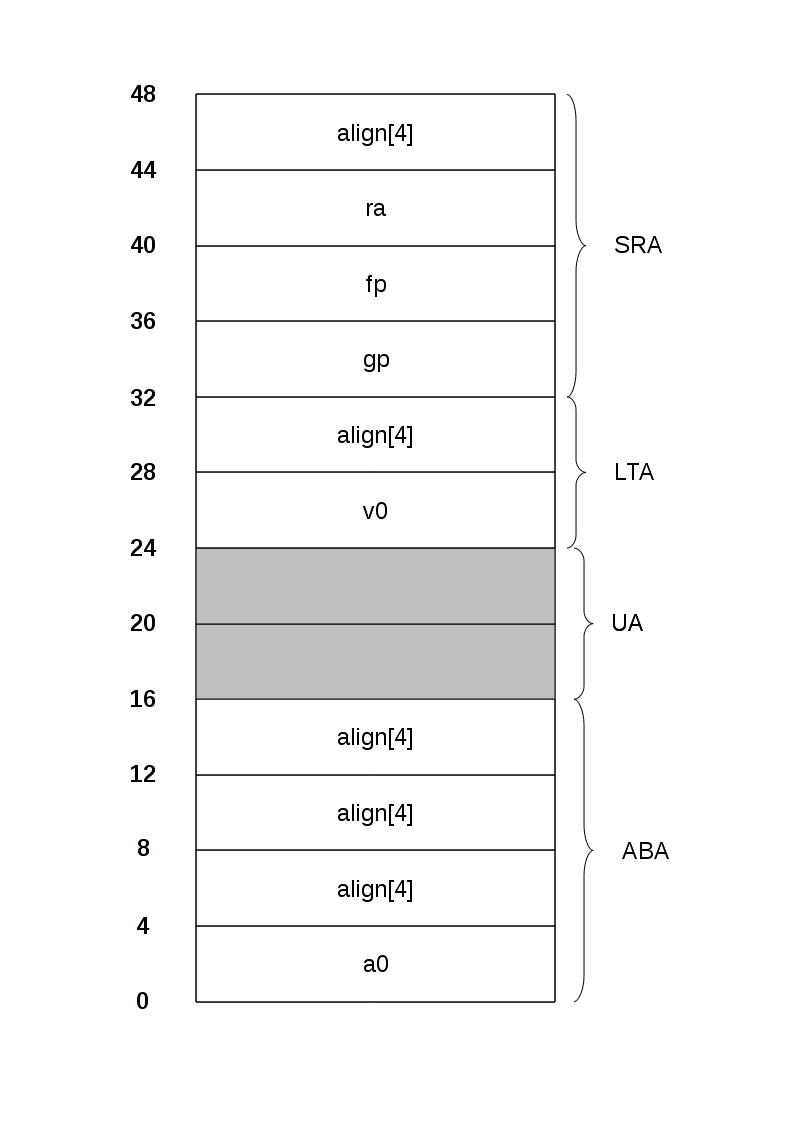
\includegraphics[width=10cm, height=15cm]{DibujosStackFrame/stack-traducirFormato.jpg}
      \end{center}

 
\section{Preparando el ambiente para NetBSD}
 
\section{Compilando en NetBSD}

\section{Ejecutando los programas en NetBSD}

\section{Casos de prueba}

\newpage
\section{Conclusiones}
  TODO

%APENDICES
\appendix
\newpage
\section{C\'odigo Fuente}
  \subsection{C\'odigo en C}
    \subsubsection{unix2dos.c}
      \lstset{numbers=left, frame=single, breaklines=true}
      \lstinputlisting{../../Tp0/Codigo/unix2dos.c}
    \subsubsection{dos2unix.c}
      \lstset{numbers=left, frame=single, breaklines=true}
      \lstinputlisting{../../Tp0/Codigo/dos2unix.c}
    \subsubsection{conversor.c}
      \lstset{numbers=left, frame=single, breaklines=true}
      \lstinputlisting{../../Tp0/Codigo/conversor.c}
  \newpage
  \subsection{C\'odigo en Assembly}
    \subsubsection{unix2dos.S}
      \lstset{numbers=left, frame=single, breaklines=true}
      \lstinputlisting{../src/unix2dos.S}
    \subsubsection{dos2unix.S}
      \lstset{numbers=left, frame=single, breaklines=true}
      \lstinputlisting{../src/dos2unix.S}
    
\newpage
\section{Enunciado}
%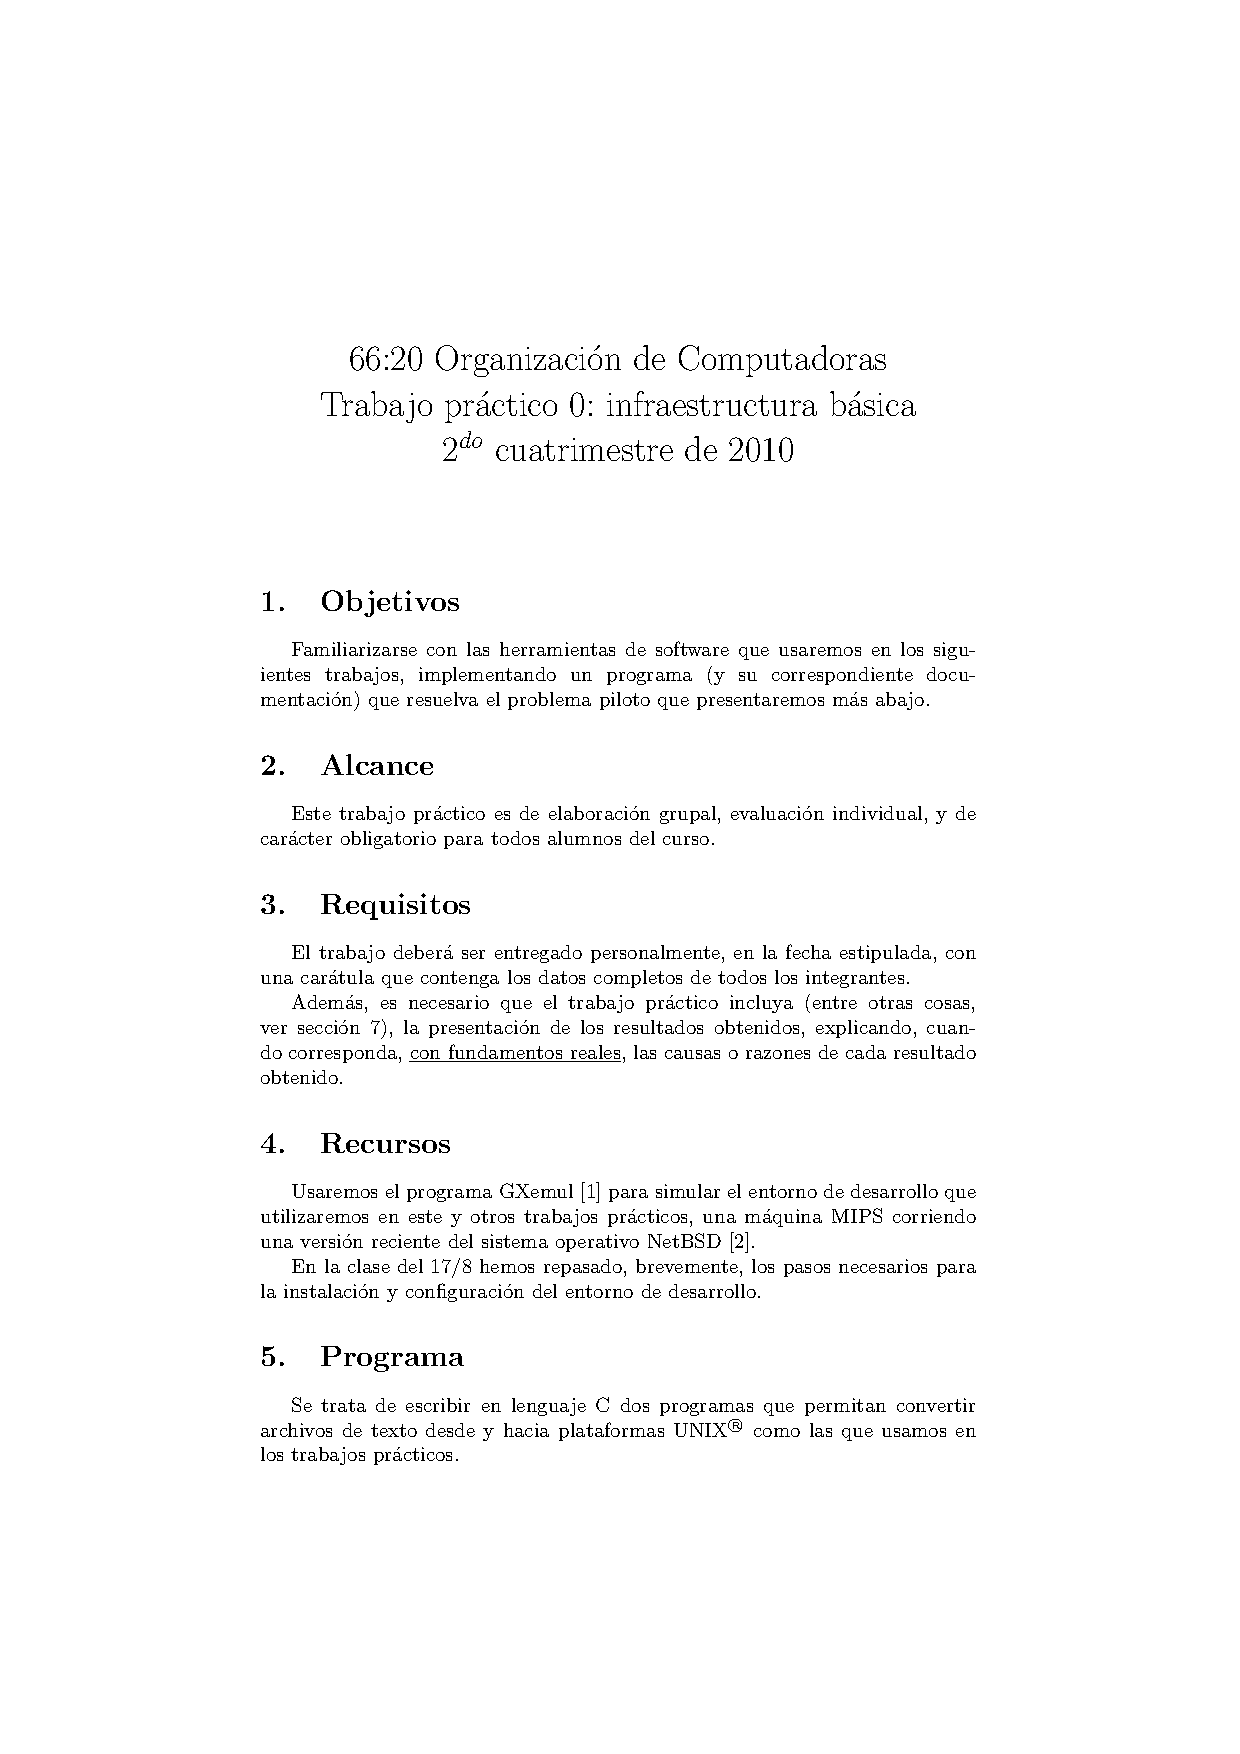
\includepdf[pages=1-3, scale=0.9, pagecommand={\thispagestyle{plain}}]{../tp0-2010-2q.pdf}

\end{document}
